\justifying
\NSFCBodyText

\subsubsection{项目特色}

本项目的第一个特色，是\textbf{把力气花在检查前提上}。

遥感图文检索的主流路径是让对齐更细、让表示更强。本项目不在这条路径上继续加码，而是退回到更靠前的位置发问：当文本描述本就不可能覆盖影像全部内容时，"未配对即为负例"这一对比学习的默认假设还成立吗？研究对象由此从"如何对齐得更好"转为"哪些监督信号是有依据的"。

第二个特色是\textbf{把可证伪性写进方案}。本项目的核心假设有明确依据：遥感基准为每幅影像配置多条互补描述这一构建方式本身，就说明单条描述不足以覆盖影像内容\cite{lu2018rsicd,yuan2022amfmn}；而现有失配处理方法确实不区分失配成因\cite{pmpguard2026,hu2023rcl}。在此基础上，本项目仍为三条假说各自设定了证伪条件，并把 H1 的检验前置到第一年——依据充分不等于结论已定，把检验放在最前面，是为了让方案在任何结果下都能继续推进。这使得项目结论无论正负都具有信息量。

第三个特色是\textbf{证据纪律}。训练端允许使用自动抽取的弱标注，评测端坚持人工核验；标准检索、关系挑战、迁移测试分别报告；改动过真值的评测绝不与原论文数字直接比较。这些约束会让最终报出来的数字更保守，换来的是结论可被他人复现与检验。

\subsubsection{创新点}

\begin{enumerate}
    \item \itemtitlefont{把"关系证据的可判定状态"作为一等建模对象。}现有引入实体与空间关系的遥感检索工作以关系增强表示与对齐为目标\cite{zhang2023unimodal,shui2025esrn,wu2024scat,yang2024dove,mi2024knowledgeaware}；现有处理图文失配的工作则把不匹配作为单一噪声统一抑制或重加权，不区分成因\cite{hu2023rcl,han2023msc,yang2023bicro,zhang2024npc,feng2024tripartition,pmpguard2026}。本项目将"这条关系在影像中能否被判定"从隐含前提提升为显式建模变量，区分"已支持""明确冲突""未知"三态，并使只有前两态参与监督。其科学意义不在于增加一个网络模块，而在于修正跨模态对齐中一个被默认接受的前提——它直接决定负样本从何而来。

    \item \itemtitlefont{以描述不完备性驱动关系约束与配套评测协议。}本项目利用同一影像多条描述之间的覆盖差异作为天然监督信号，无需额外人工标注即可获得初始的三态线索；并配套构建经人工核验的关系挑战评测与覆盖度分档稳健性评测，使"关系建模是否真的起作用"可被独立检验。其科学意义在于把"描述不完备"从数据缺陷重新定位为\textbf{可利用的结构性信息}，同时给出使结论可归因的验证设计。
\end{enumerate}

\subsubsection{与最相关工作的差异说明}

需要明确的是，空间关系增强与不完备图文对应\textbf{均已有成熟研究}，本项目不作任何"首次"或"填补空白"的主张。与最相关工作的差异如下：

面向遥感伪匹配对的 PMPGuard\cite{pmpguard2026} 以高斯混合模型拟合匹配与不匹配的相似度分布并学习判定边界，判定的是失配程度而非失配成因，也未显式建模空间或实体关系；本项目区分失配成因，并让未知态不参与负样本监督。面向遥感图文检索的空间感知实体关系探索\cite{shui2025esrn} 与实体关系的单模态特征学习\cite{zhang2023unimodal} 侧重关系增强的表示与对齐，本项目侧重关系证据的状态判定与未知态处理。通用领域中不确定性与证据建模的工作\cite{chun2021pcme,han2021tmc,li2023pau,qin2022decl} 建模的是相似度或表示的不确定性，本项目建模的是关系命题的可判定状态——技术手段可以借用，问题定义并不相同。 图~\ref{fig:positioning}从关系语义和失配处理两个维度归纳上述差异。

% F9: F09_差异定位.png
\begin{figure}[!htbp]
    \centering
    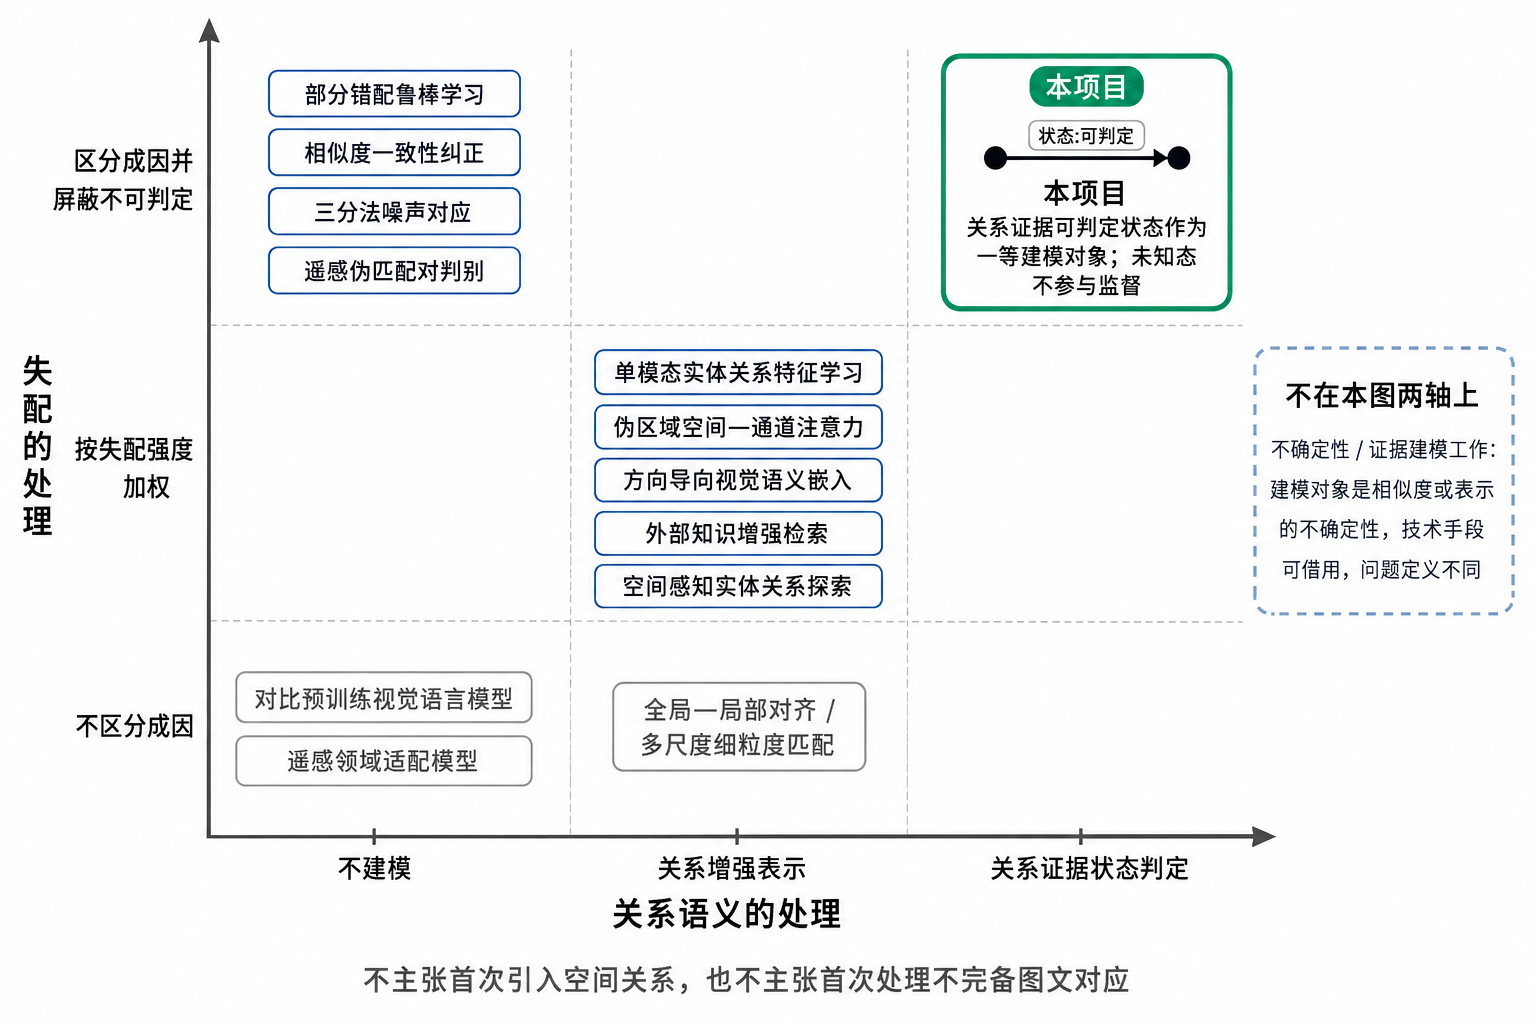
\includegraphics[width=\linewidth]{figures/F09_差异定位.png}
    \caption{与最相关工作的差异定位。两轴为方法处理方式的定性归纳，节点位置不表示性能排名。}
    \label{fig:positioning}
\end{figure}


本项目的创新主张因此限定为：\textbf{把关系证据的可判定状态作为跨模态匹配中的一等建模对象，研究仅对可核验关系施加约束、对未知关系不施加监督的对齐方式，并用独立核验的关系证据检验其效果。}这是方法层面的问题重述与验证设计，不是新任务或新领域的开创性声明。
